\documentclass[border=2mm]{standalone}
\usepackage{tikz}
\usetikzlibrary{calc,patterns,angles,quotes}
\begin{document}
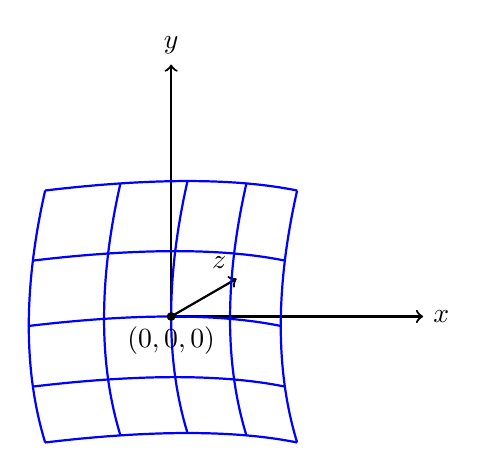
\begin{tikzpicture}[scale=0.8, declare function={f(\x,\y)=\y*\y/4-\x*\x/4;}]
% Vẽ trục tọa độ
\draw[->, thick] (0,0) -- (4,0) node[right] {$x$};
\draw[->, thick] (0,0) -- (0,4) node[above] {$y$};
\draw[->, thick] (0,0) -- ({0.3*4*cos(30)},{0.3*4*sin(30)}) node[above left] {$z$};

% Vẽ các đường cong ứng với x cố định (parabol theo y)
\foreach \x in {-2,-1,0,1,2} {
    \draw[blue, thick, smooth] plot[variable=\y, domain=-2:2, samples=30] ({\x + 0.3*f(\x,\y)*cos(30)}, {\y + 0.3*f(\x,\y)*sin(30)});
}
% Vẽ các đường cong ứng với y cố định (parabol theo x)
\foreach \y in {-2,-1,0,1,2} {
    \draw[blue, thick, smooth] plot[variable=\x, domain=-2:2, samples=30] ({\x + 0.3*f(\x,\y)*cos(30)}, {\y + 0.3*f(\x,\y)*sin(30)});
}

% Đánh dấu điểm yên
\fill (0,0) circle (2pt) node[below] {$(0,0,0)$};
\end{tikzpicture}
\end{document}